\chapter{Progress}

Budd's sliding theory examines how stress propagates through an ice mass as it flows over an undulating bed. When ice encounters a bedrock bump, it creates a complex stress field that propagates upward through the ice column at an angle rather than vertically, (see figures \ref{fig:P} for the pressure and \ref{fig:Vx} horizontal velocity fields). The steady-state surface shape consists of waves similar to the bedrock perturbations but out of phase by approximately $\pi$. As a direct mathematical consequence, ``the steepest slope occurs over the highest bedrock''\cite{Budd_1970} not the surface undulation itself. To verify Budd's sliding law, this simulation implements a flowband model across a 10 km domain with 100 m resolution. The simulation features an 800 m mean ice thickness over bedrock at 1 km elevation, with a -0.1 radians downward slope in the x-direction and imposed cosine undulations (2.64 km wavelength, 0.1 km amplitude). The main model, executes a 300-year transient Full-Stokes simulation using 1-year time steps. The current implementation demonstrates the stress propagation through ice flowing over spatially varying basal friction according to a simplified version of Budd's sliding law (see figure \ref{fig:Friction}) and validates the non-linear rheology (n = 4.0) that I use.


% surface undulations phase-shifted by $\pi$/2
\begin{figure}[H]
    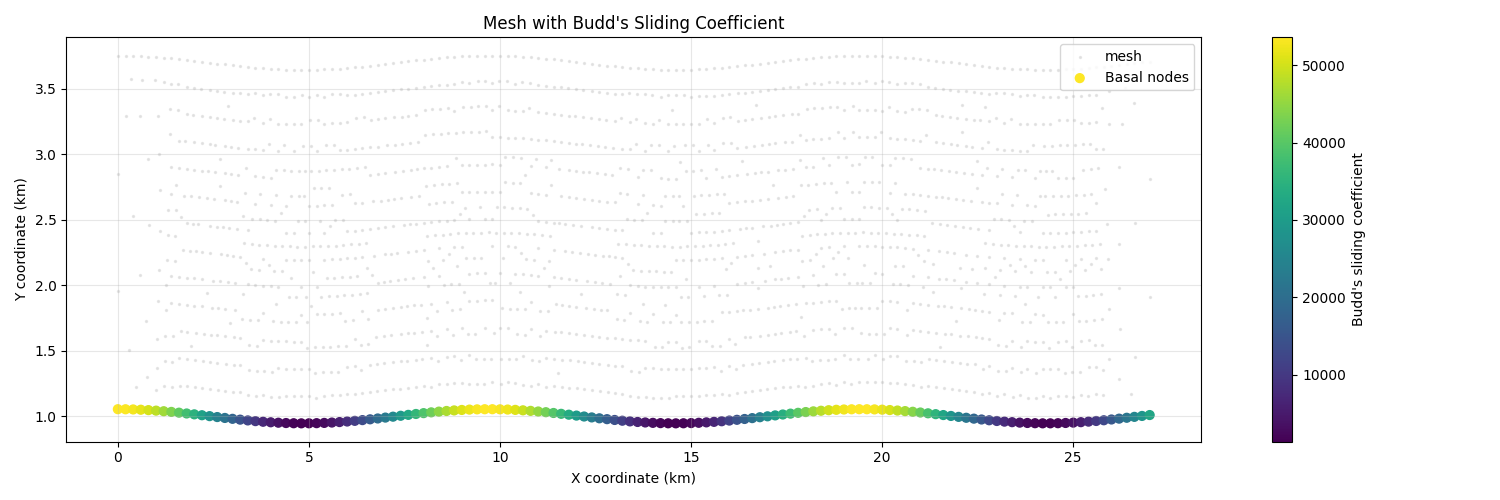
\includegraphics[scale=0.5]{basal_friction.png}
    \caption{Slope parallel visualisation of the computational mesh with basal nodes highlighted. The gray dotted lines represent the complete finite element mesh with multiple vertical layers conforming to the undulating geometry. Basal nodes (yellow to purple) follow the periodic undulated bed topography. The colour gradient along the basal nodes display the imposed variations in basal friction coefficient implemented through a simplified version of Budd's sliding law, with lighter colours indicating regions of higher basal drag es per Budd's sliding theory.}
    \label{fig:Friction}
\end{figure}


\begin{figure}
    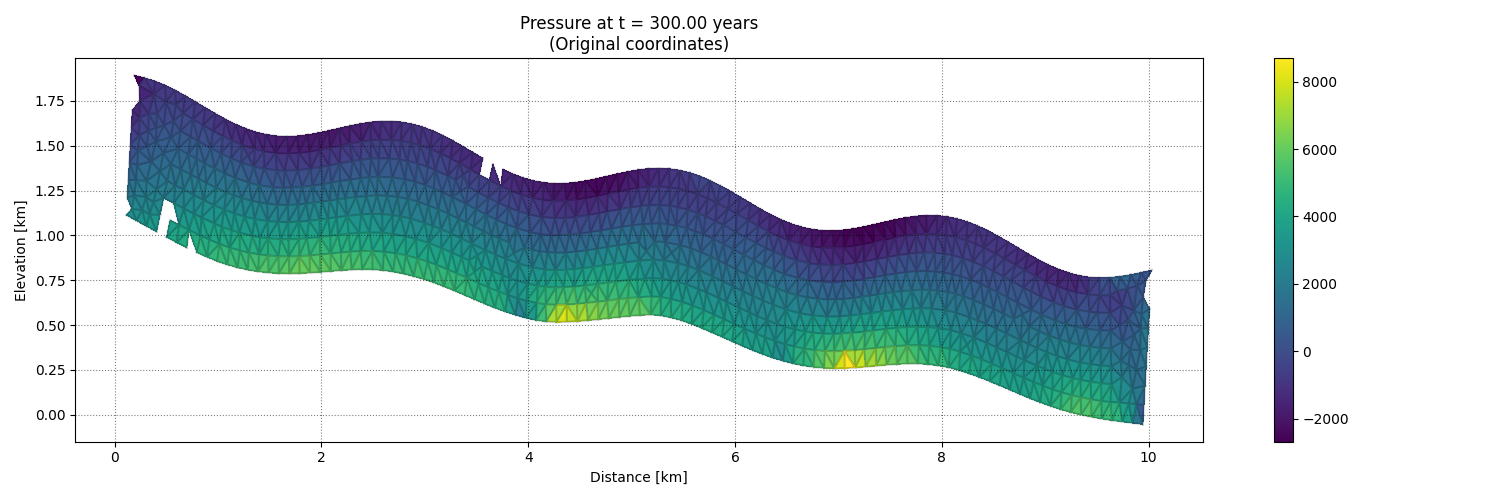
\includegraphics[scale=0.45]{Pressure_300yrs_xz.png}
    \caption{Pressure field distribution at t = 300.00 years shown in original coordinates. The color scale (ranging from -2000 to 8000 Pa) reveals the spatially distributed pressure variations throughout the ice body, with higher pressures (yellow) concentrated before the peaks of the bed undulations. The triangular mesh elements display the finite element discretisation used for solving the Stokes equations. The development of low-pressure zones near the surface aligning with the undulating basal topography suggests stress transfer from the imposed variation in basal friction. Note: The white gaps visible within the mesh represent masked areas excluded from visualization processing, not physical features or data gaps in the original simulation.}
    \label{fig:P}
\end{figure}

\begin{figure}
    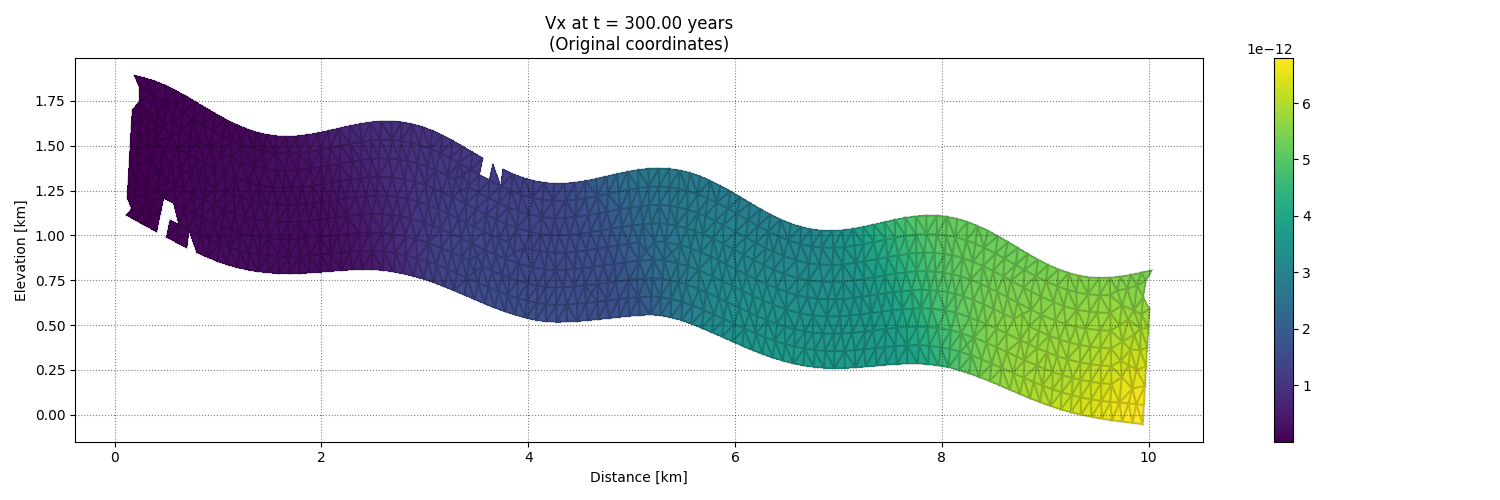
\includegraphics[scale=0.45]{Vx_300yrs_xz.png}
    \caption{Horizontal velocity field ($V_x$) at t = 300.00 years displayed in original coordinates. The color scale indicates velocity magnitude ($10^{-12}$ km/s, equivalent to $\approx 31.5$ mm/year at the maximum) with flow direction from left to right. The velocity pattern shows clear acceleration as the ice flows downslope, with highest velocities (yellow) occurring near the terminus. The fixed upstream boundary condition  constrains flow at the inlet, while the progressive acceleration downstream results from gravitational forcing along the sloped bed. Note: The white gaps visible within the mesh represent masked areas excluded from visualization processing, not physical features or data gaps in the original simulation.}
    \label{fig:Vx}
\end{figure}

\begin{figure}
    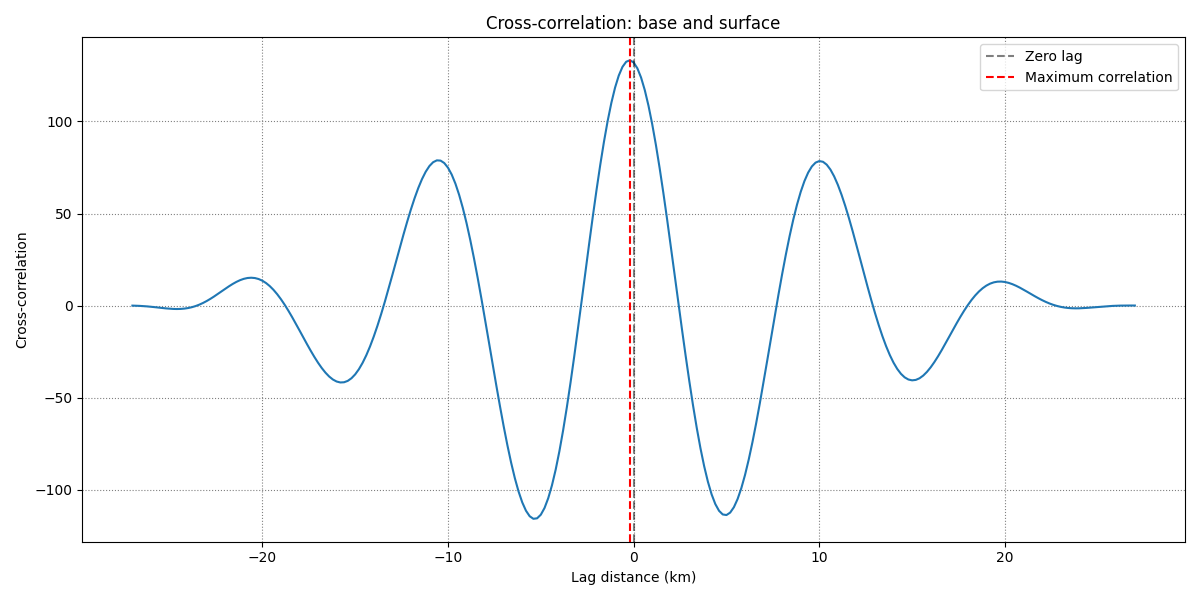
\includegraphics[scale=0.5]{xcorr.png}
    \caption{Cross-correlation between the base and surface slope signals across spatial lags. The maximum correlation corresponds to the lag distance of 0.7 km, which translates to a phase shift of 0.53$\pi$ (95.5 degrees), only 0.03$\pi$ radians away from Budd's theoretical value.}
    \label{fig:xcorr_filtered}
\end{figure}

\begin{figure}
    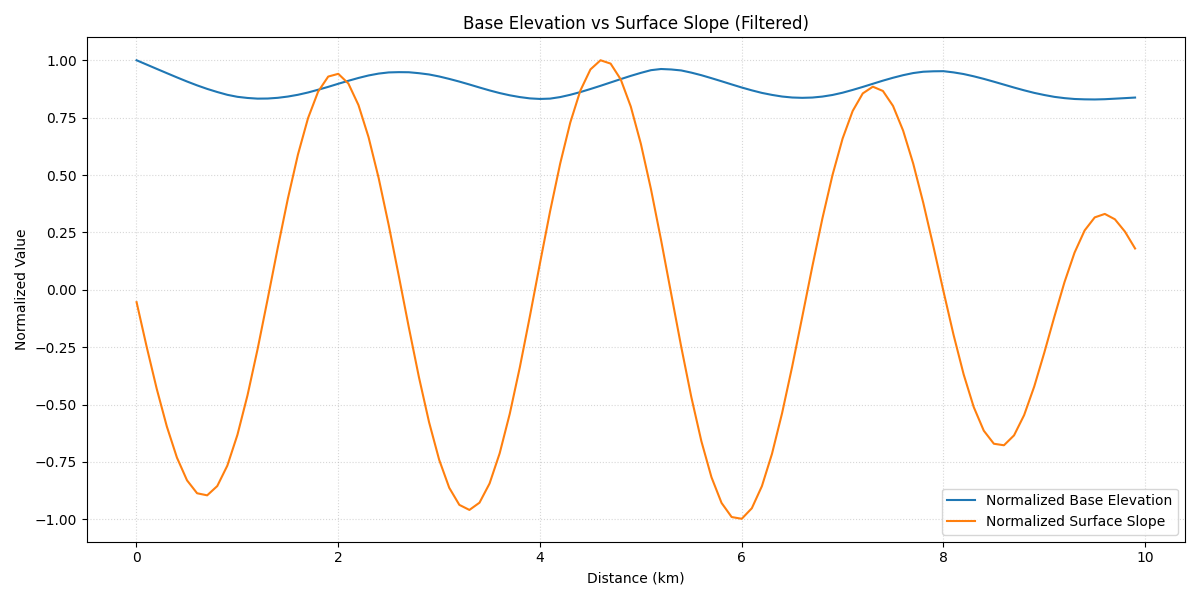
\includegraphics[scale=0.5]{direct.png}
    \caption{Visual comparison of topographic profile of bedrock compared to the surface slope signal in slope-parallel coordinates. Here it is clearly visible that the surface slope (orange) is shifted to the right of the peak in bed elevation (blue), with approximately the predicted phase shift. This result is strong evidence that my simple model is correctly capturing the physics described in Budd's paper. The surface slope is responding to bed undulations with the expected phase relationship - maximum surface slopes occur slightly downstream of the highest bed elevations.}
    \label{fig:direct}
\end{figure}












